% Chapter 5
\chapter{Anomaly Detection} % Main chapter title

\label{Chapter5} % Fr referencing the chapter elsewhere, use \ref{Chapter1} 

\lhead{Chapter 5. \emph{Anomaly Detection}} % This is for the header on each page - perhaps a shortened title

%----------------------------------------------------------------------------------------
\section*{Overview}
In this chapter, we use clustering property of diffusion maps together with multiscale approach based on Laplacian pyramid representation for anomaly detection in images. It is expected that diffusion maps clusters the background pixels, and thus in new embedding, the anomaly is far from the clusters. The presented algorithms is tested  on simple to complex images to prove its effectiveness or failures.

%----------------------------------------------------------------------------------------
\section{Introduction}
\label{C5:Intro}
Anomaly detection refers to the problem of finding patterns in data that do not conform to expected behavior. In computer vision anomaly detection algorithms rely of course on complex image processing methods as a preprocessing step to separate the anomalous points from the background of
an image. The large dataset, the presence of noise and high dimensionality of the data makes the anomaly detection in images a challenging task.

The stimulating task of anomaly detection have been studied by many researchers over the past decades. A review paper \citep{Pime2014}  tries to provide a structured and comprehensive overview of the research on anomaly detection by extracting six approach namely probabilistic, distance-based, domain-based, dimension reduction, reconstruction-based,  and information theoretic approach. The dimension reduction and reconstruction based approach   is one quite useful in anomaly detection. Such techniques can find a representation which separates the anomaly from the background. Adding to the same, the former being data driven approach doesn't depends on the model, training data and the choice of the distribution. In contrast to the well-known above classification setup, Goldstein and Uchida \citep{Gold2016} have classified anomaly detection approaches based on labels available in the dataset as illustrated in figure \ref{anomaly}. In our paper, as we have unlabeled data, we use unsupervised algorithms.

\begin{figure}[ht]
\begin{center}
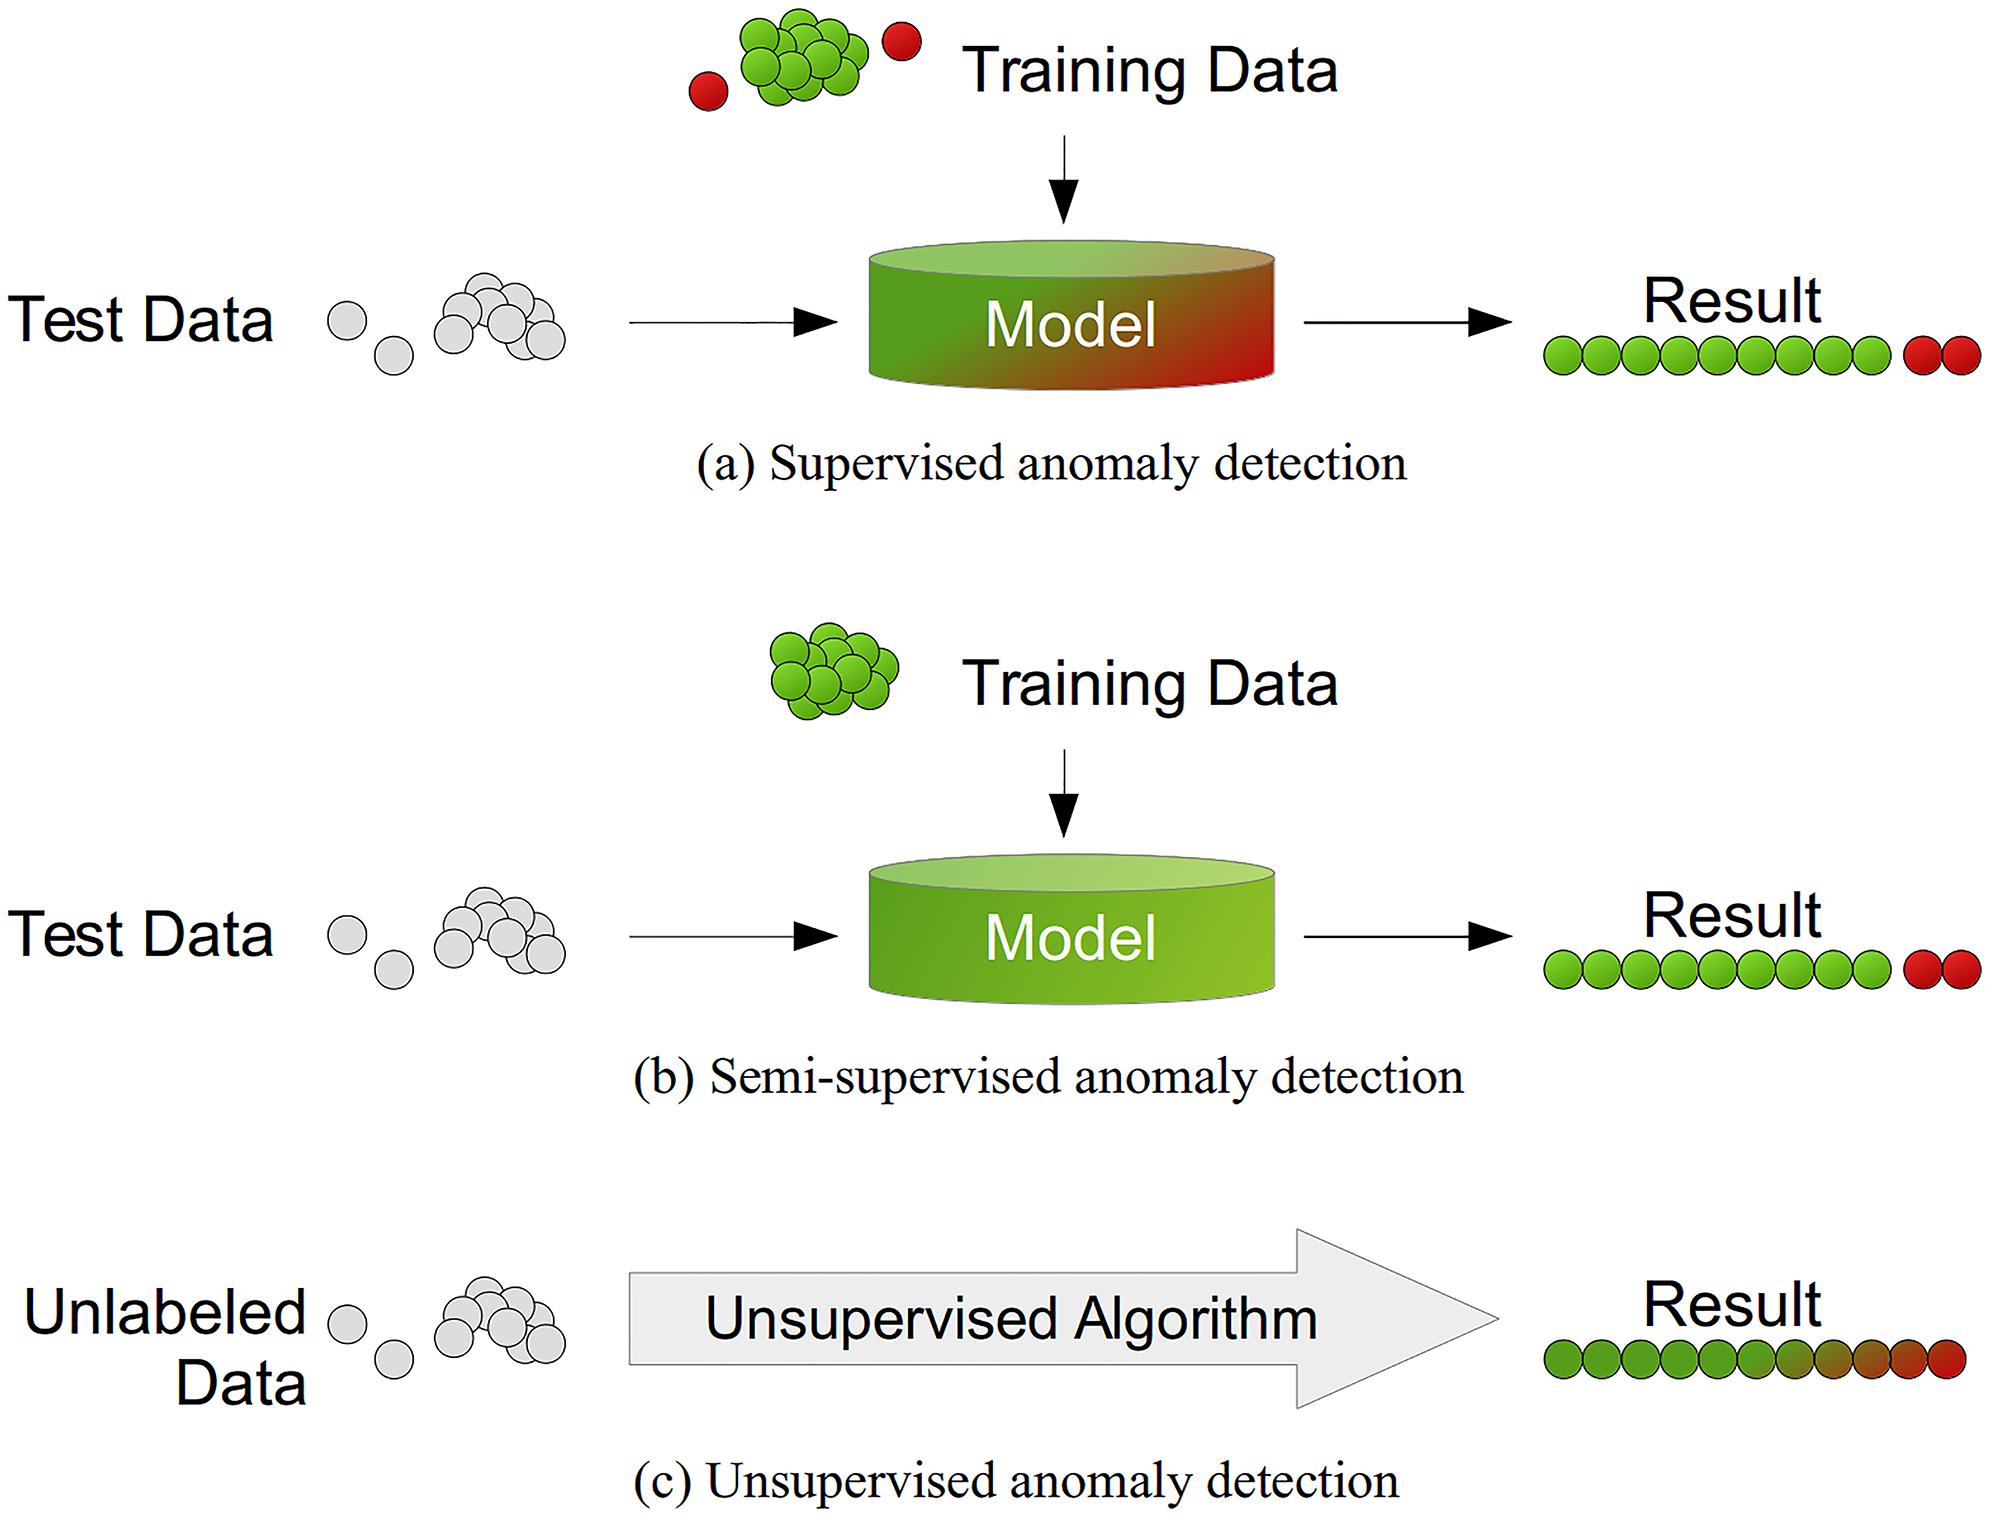
\includegraphics[width=\textwidth]{./Figures/anomaly.png}
\caption {Anomaly detection approach based on data labels.}
\label{anomaly}
\end{center}
\end{figure}

Though, there is girth of approach using manifold learning algorithms, a convincing generic approach for anomaly detection still searching for best fit. 

Motivated by the Mishne and Cohen paper \citep{Gal2013}, we use manifold learning approach, in particular, diffusion maps combining spectral dimensionality reduction and a nearest-neighbor-based anomaly score to detect anomaly in the images. The Laplacian pyramid representation a integral part of our approach which take care of problems associated with interpolative nature of extension methods used by diffusion maps.

\section{Diffusion Maps}
\label{dfm}
Diffusion map is a manifold learning method that maps high-dimensional data to a low-dimensional diffusion space by constructing the graph Laplacian of the data set.

Considering high dimensional data $\mathbf{X}=\{x_1, x_2, x_3, ..., x_N\}\in \mathbb{R}^{N\times\mathbf{D}}$, we construct a weighted graph. Where, the data points are the nodes and edge weight is similarity measure between the two data points. With suitable weight function, we create random walk by by normalizing the kernel. Now using spectral decomposition of matrix created by random walk, we compute diffusion distance using eigendecomposition. As the spectrum decays really fast, we get reduced dimension embedding. The details mathematical description of diffusion maps is discussed in Chapter \ref{Chapter3} (\ref{s:dm}).

The scale parameters ($\sigma$) defined in Gaussian kernels  $w(x_{i},x_{j})=\exp(-\Vert x_{i}-x_{j}\Vert^{2}/\sigma^{2})$ for constructing the weighted graph is very important. Setting $\sigma$ to be too small results local neighborhoods of size 1. Large $\sigma$ connect the anomalies with the cluttered background. In our paper, we use  location dependent $\sigma$ for each data point instead of selecting a single scaling parameter as discussed in \citep{Gal2013}. The scale $\sigma$ is calculated for the neighborhood of point statics $x_{i}$, for example, $\sigma_{i}=\Vert x_{i}-x_{K}\Vert^{2}$. Then, the similarity kernels are calculated as $w(x_{i},x_{j})=\exp({-\Vert x_{i}-x_{j}\Vert^{2}\over\sigma_{i}\sigma_{j}})$.

\section{Function Extension}
It is impractical to compute a diffusion map for the large dataset. Instead, a diffusion map is constructed for part of the samples.The embedding is then extended to all points using an out-of-sample extension method. The algorithms for one such out-of-the sample method is done using Laplacian Pyramid \citep{Gal2013}.

\section{Laplacian Pyramid}
\label{C5:LP}

The Laplacian pyramid algorithm constructs a coarse approximation of a function $\mathbf{f}$ for a given scale at each iteration. 
In the next iteration, we use the difference between $\mathbf{f}$ and the coarse approximation as input, which is approximated as Gaussian kernels at each level with scale getting finer and finer.

We define Gausian Kernels on $\mathbf{X}$ at lowest level as:
\begin{equation}
\mathbf{W}_{0}^{L}\buildrel{\Omega}\over{=}w_{0}^{L}(x_{i},x_{j})=\exp(-\Vert x_{i}-x_{j}\Vert^{2}/\varepsilon_{0})
\label{lp:1}
\end{equation} 
where $\varepsilon_{0}\gg$. Normalizing $\mathbf{W}_{0}^{L}$ in equation \ref{lp:1}, we get smoothing operator $\mathbf{Q}_{0}^{L}$

\begin{equation}
\mathbf{Q}_{0}^{L}=q_{0}^{L}(x_{i},x_{j})=(q^{L}_{0})^{-1}w_{0}^{L}(x_{i},x_{j})
\end{equation}

where $q^{L}_{0} = \sum_{j}w_{0}^{L}(x_{i},x_{j})$. Similar construction is done for the next level to get $\mathbf{W}^{L}_{l}, \mathbf{Q}^{L}_{l}$. Using this iteration, we get the Laplacian Pyramid representation $\mathbf{f}$ of $\mathbf{X}$, which is then iterated on finer and finer scales until the
difference between function $\mathbf{f}$ and approximation is below some error threshold. For mathematical details, please see \citep{Gal2013}.

\section{Multiscale Anomaly Detection}
\label{C5:MS}
The method motivated from base paper\citep{Gal2013} overcomes the limitations of random sampling with a multiscale approach. In reality, it is not hard to believe that the anomalies in the image are larger than a single pixel, which is hard to be detected at several resolutions of the image. The situation is much worst at lower resolution. As it is impossible to sample a larger percentage of the lower resolution image, the anomaly detection is bound to fail. Multiscale  approach  overcome the limitations of random sampling by performing anomaly detection at different resolutions of the image, which gets finer and finer if any anomaly is missed. The Laplacian pyramid representation of the image is constructed starting from coarsest scale giving rise diffusion map using subset of the data or even whole pixel. Anamoly score is used at this level to determine which pixel is anomaly. Using this pixel as input to the next coarser level to detect next anomalous pixel. It is then continued from level to level, with each previous level providing prior information on which samples of the data set are used to construct the diffusion map. In the next section, we present the algorithms in the detail.

\subsection{Algorithms}
\label{C5:Imp}
\begin{enumerate}
\item Input Image: $\mathbf{I}$. Size: $400\times400$.
\item For $l = 0:L$ compute Gaussian pyramid $\{\mathbf{G}_{i}\}^{L}_{l=0}$, where $\mathbf{G}_{0}$ is the original image and $\mathbf{G}_{L}$ is the coarsest resolution as discussed in section \ref{C5:LP}.
\item Starting with $\mathbf{G}_L$, sample a subset $\mathbf{I}_{s}$ from $\mathbf{I}$.
\item Compute Diffusion map using $\mathbf{I}_{s}$. 
\item Extend above step to remaining pixels.
\item Calculate anomaly score $\mathbf{C}_l$ for $400\time400$ pixels.
\item Set threshold $\tau_{l}$ to 95th percentile of the anomaly score.
\item If $\mathbf{C}_l > \tau_{l}$, the anomaly will be sampled more densely. Goto step 2, else 
\item output.
\end{enumerate}
 
We then sample the rest of the  pixels randomly. In the anomaly score $\mathbf{C}_{l-1}$ calculated, anomaly gets high score, separating it from the background. The algorithms is illustrated using flowchart \ref{algo}.

\begin{figure}[ht]
\begin{center}
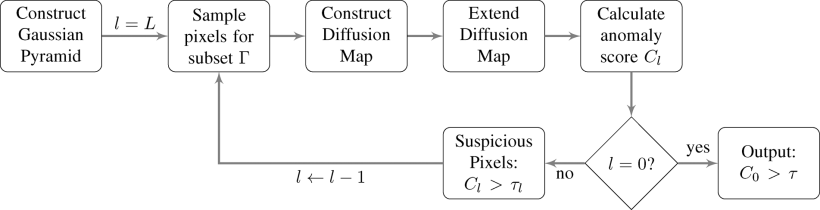
\includegraphics[width=\textwidth]{./Figures/algo.png}
\caption {Multiscale Algorithm.}
\label{algo}
\end{center}
\end{figure}

The affinity matrix at each level is calculated for subset of $\mathbf{X}_l$ using $w(x_{i},x_{j})=\exp({-\Vert x_{i}-x_{j}\Vert^{2}\over\sigma_{i}\sigma_{j}})$ with scaling parameter as explained in section \ref{dfm}. The nearest neighbors is used to calculate matrix to reduce computation time and memory requirements. This makes the matrix sparse. The anomaly score for each level is  based on a nearest-neighbor approach too. 

To determine any pixel as anomaly, we define anomaly score of tested pixels $i$ using below equation.

\begin{equation}
\mathbf{C}_{l}(i)=1-{1\over m}\sum_{j\in N_{i}}\overline{w}(i,j)
\end{equation}

where $m$ is the number of pixels in $N_i$.

We compare pixel $i$ to its neighbors $\{j\}$ in the spatial neighborhood denoted by $N_{i}$, which is a square window surrounding pixel $i$ of size $2\mathbf{W}+1$ in each dimension. As, we assume that anomaly is larger than a pixel, we mask the inner part of the window surrounding the tested pixel. We use only the pixels in the outer window.

The smoothed estimate of the number of close neighbors $i$ is defines as $\sum_{j\in N}\overline{w}(i,j)$. The notion of closeness is determined by the diffusion distance.

\section{Data}
\label{C5:Dat}
For our experiments with the proposed algorithms, We take pictures of varied size ranging from $800\times800$ to $200\times200$. The pictures are of low resolution to contrast resolution, so that performance of the proposed algorithms can be compared. This also allow us to play with various parameters proposed in the algorithms. The figure \ref{fig:input} shows six different input image, which we consider for our experiment.
 
 
\begin{figure}[t!] % "[t!]" placement specifier just for this example
\begin{subfigure}{0.32\textwidth}
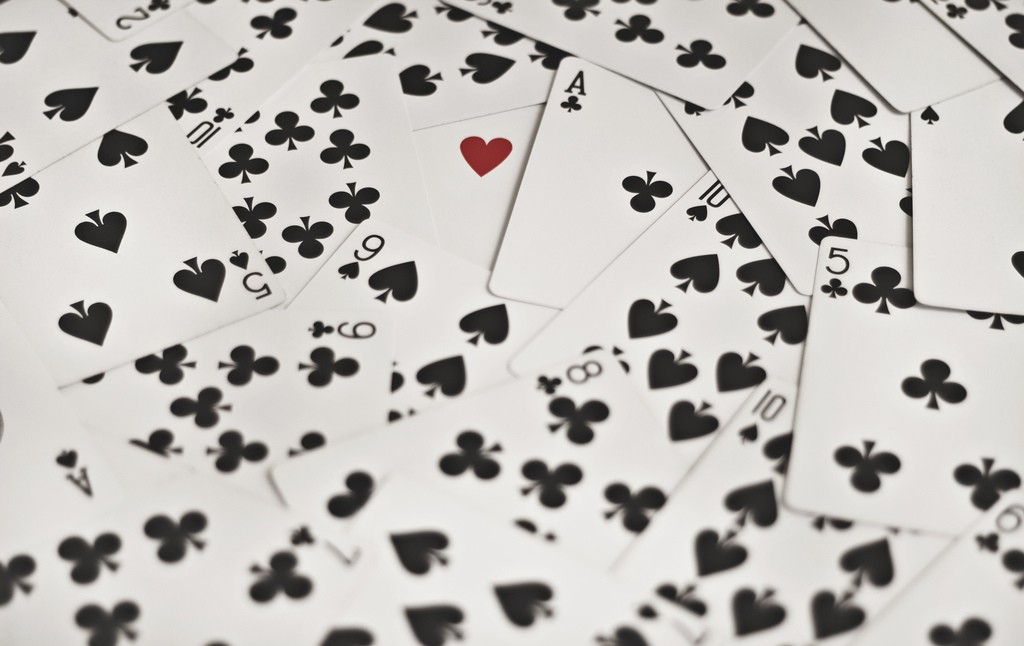
\includegraphics[height=3cm,width=3cm]{./Figures/card.jpg}
\caption{} \label{fig:a}
\end{subfigure}\hspace*{\fill}
\begin{subfigure}{0.32\textwidth}
\includegraphics[height=3cm,width=3cm]{./Figures/field.jpg}
\caption{} \label{fig:b}
\end{subfigure}
\begin{subfigure}{0.32\textwidth}
\includegraphics[height=3cm,width=3cm]{./Figures/girl.jpg}
\caption{} \label{fig:c}
\end{subfigure}

\medskip
\begin{subfigure}{0.32\textwidth}
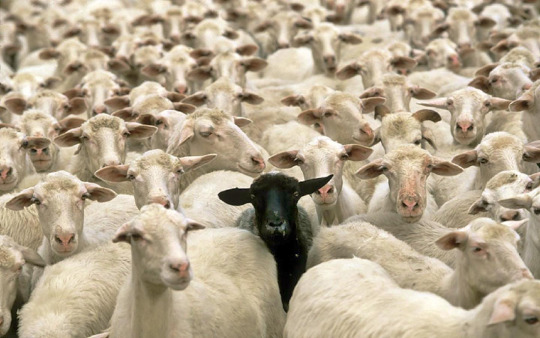
\includegraphics[height=3cm,width=3cm]{./Figures/sheep.jpg}
\caption{} \label{fig:d}
\end{subfigure}\hspace*{\fill}
\begin{subfigure}{0.32\textwidth}
\includegraphics[height=3cm,width=3cm]{./Figures/girlf.jpg}
\caption{} \label{fig:e}
\end{subfigure}
\begin{subfigure}{0.32\textwidth}
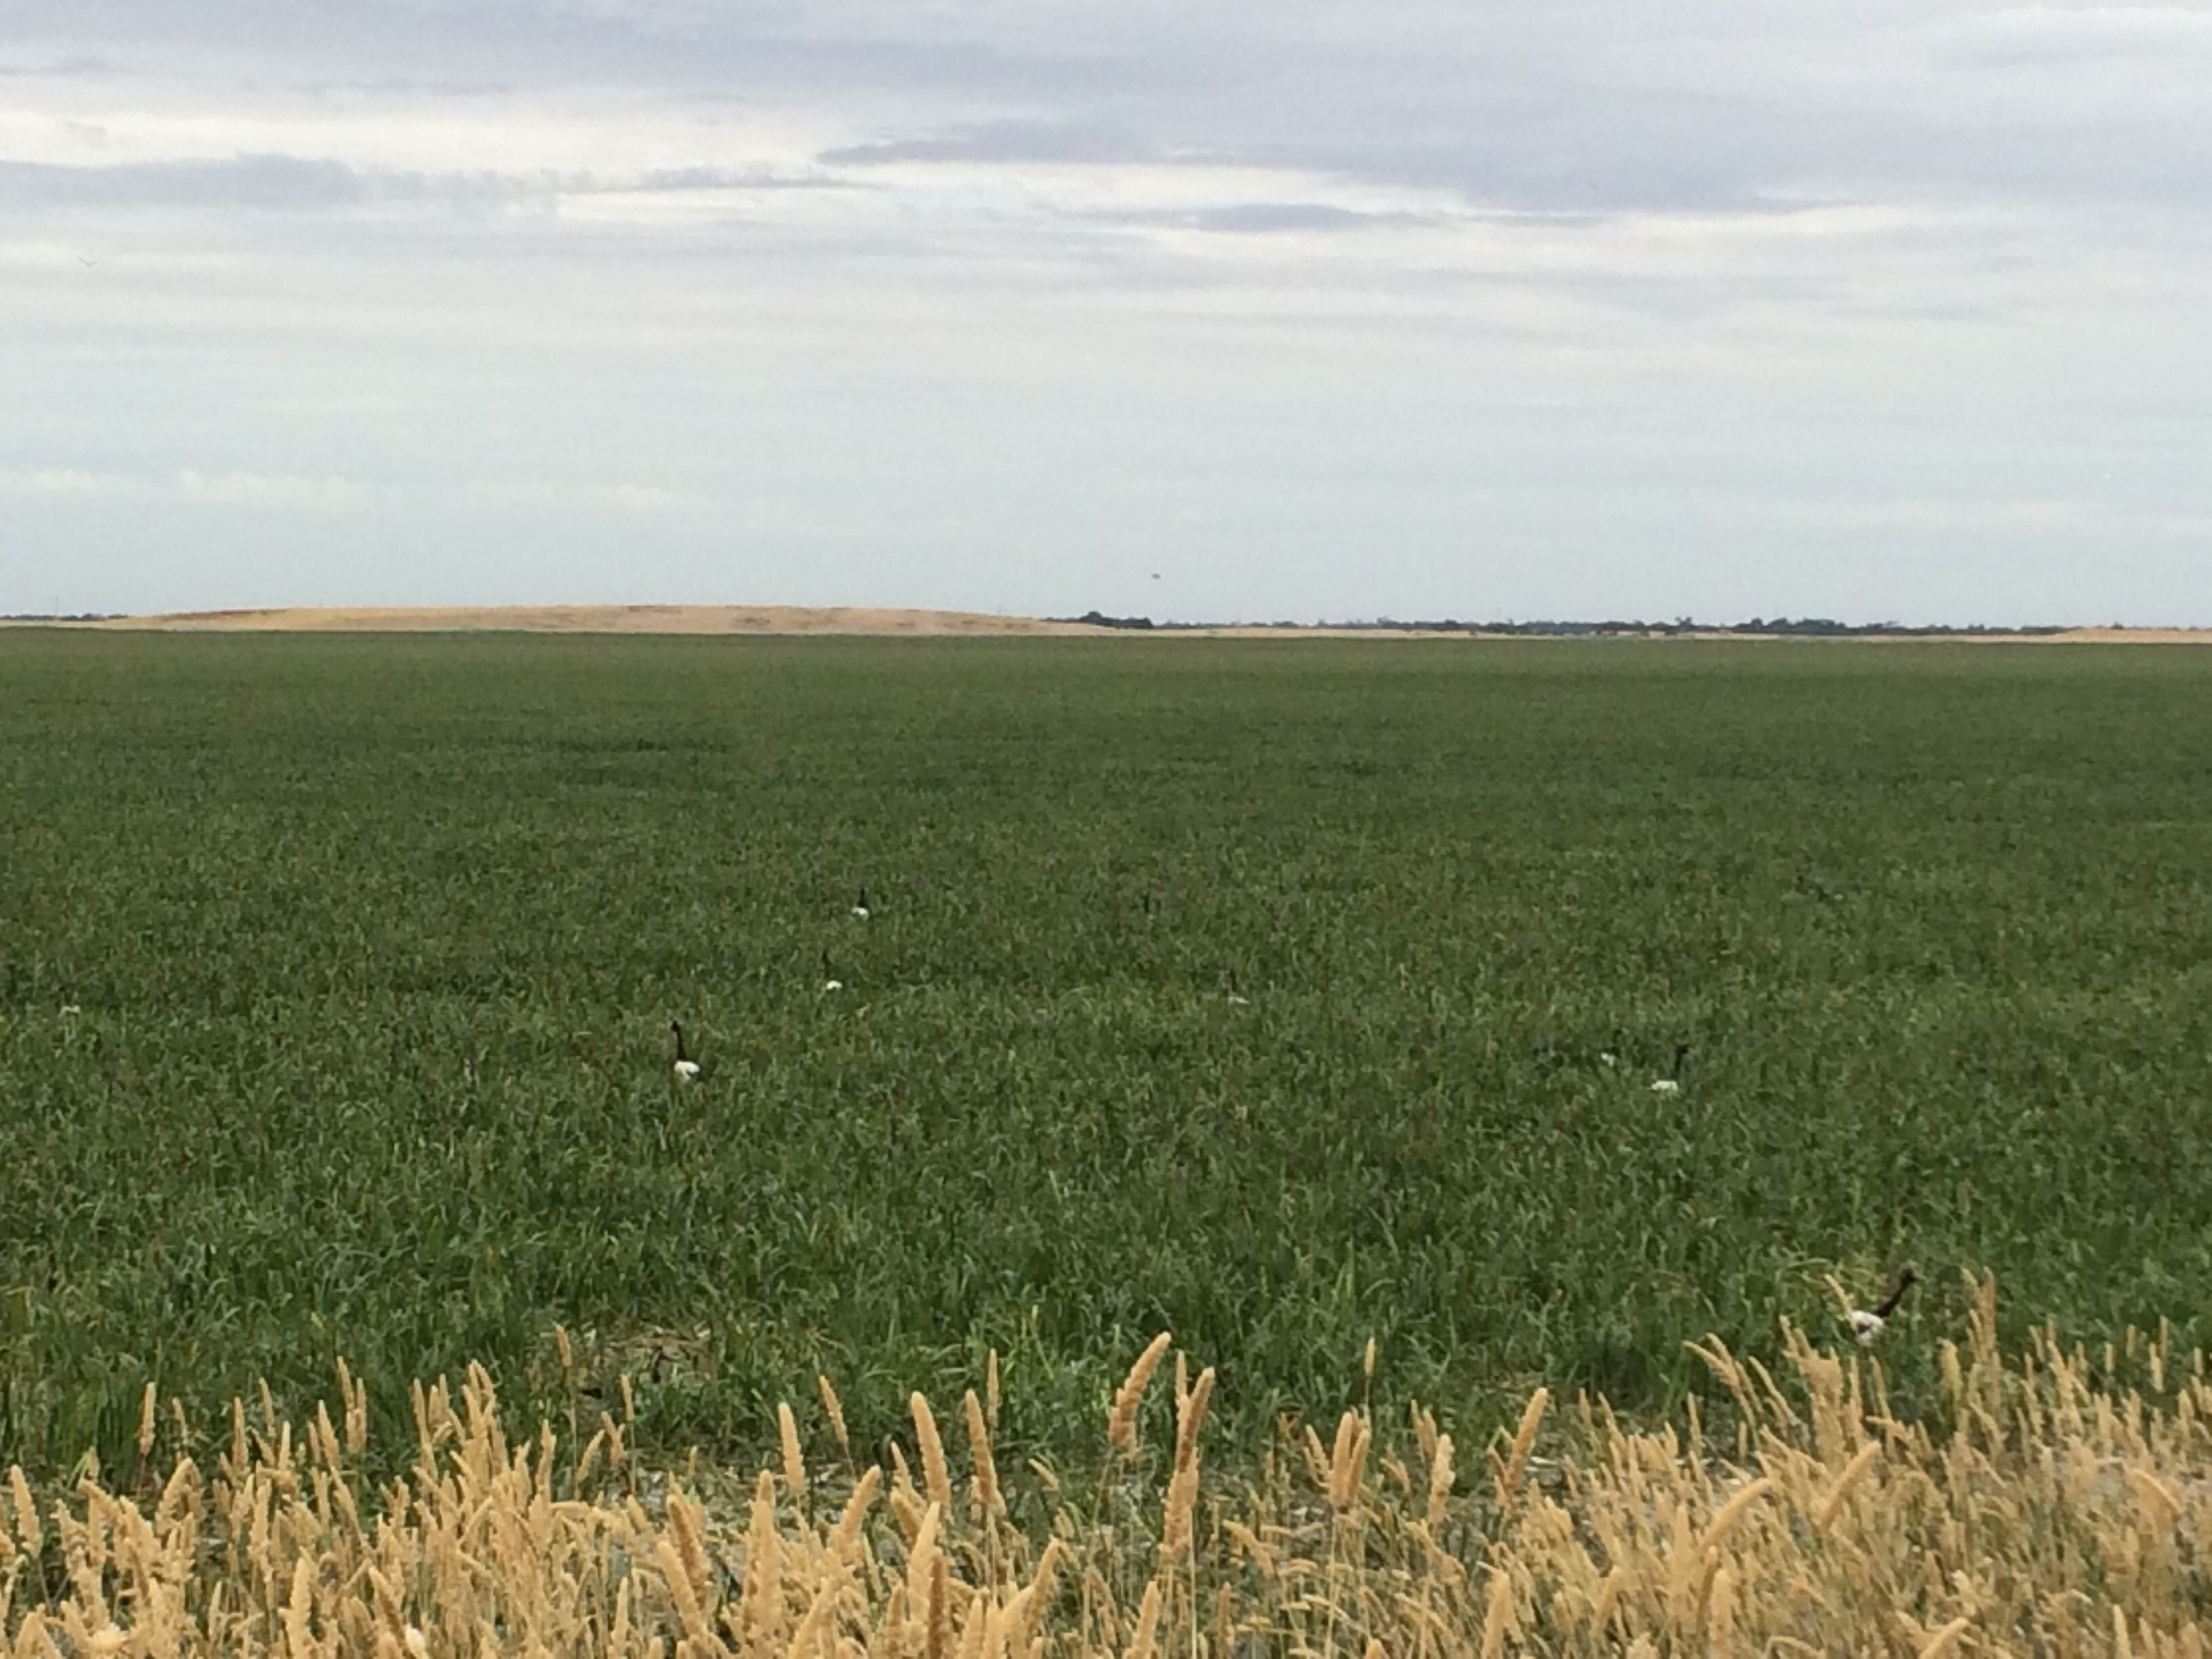
\includegraphics[height=3cm,width=3cm]{./Figures/duck.jpg}
\caption{} \label{fig:f}
\end{subfigure}

\caption{Input Image} \label{fig:input}
\end{figure}

We treat the red card in subfigure (A) \ref{fig:a}, sea-miner in subfigure (B) \ref{fig:b}, village girl in subfigure (C) \ref{fig:c}, black sheep in subfigure (D) \ref{fig:d}, girl in subfigure (E) \ref{fig:e} and duck in subfigure (F) \ref{fig:f} as anomalies. Automatic detection of anomalies is a challenging task due to the high variability in the appearance of the anomaly and background images. In the all of the pictures, the anomaly appear as a strong bright region  aside a dark region and always smaller than the background region in the image.

\section{Results}
\label{C5:Res}
Unlike other anomaly detection algorithms in the images relying on the training set, based on real images and/or synthetic ones, we just use expected size of anomalies as prior information.

The algorithms is evaluated on the all the six images, but one at a time to test the performance and results. As the pixel of images varies from $800\times800$ to $200\times200$, we set different parameters for different image. For example, we evaluated our algorithm on a set of 50 ducks in the field \ref{fig:f}, each image sized $800\times800$ pixels. As the size of our images are big compared to image used in the base paper \citep{Gal2013}, we set Gaussian pyramid level $\mathbf{L} = 5$. Starting from level zero  $\mathbf{L} = 0$, we take image size $800\times800$ pixels for input image, village girl in the field \ref{fig:f}, patch size $128\times128$ pixels, embedding dimension $\mathbf{d}=24$, percent of pixels in subset as $0.1$, window size as $64\times64$ and mask as $18\times18$. For efficient computation in all images, we calculate the affinity matrix using exact k-nearest-neighbor search with 16 neighbors for each point, resulting in a sparse weight matrix. For other levels $\mathbf{L}=1,2,3,4$, we keep decreasing the above parameters by half for each level. For the above figure, the parameters used in the multiscale detector are given
in Table \ref{T: PD}

Now, we start with basic anomaly detection for figure \ref{fig:d}. In this image, there is black sheep among white sheep. The anomaly detection results for the above input image is illustrated in the figure \ref{R:sheep}. Here, (A) represent the original image. The image detected at level 0 is depicted in (B) and its 3 dimensional coordinates in (C) through Gaussian maps embedding in (D). The (E) represents the suspicious detection leading to anomaly score in (E). The parameters used is summarized in Table \ref{T:sheep}.

\begin{figure}[t!] % "[t!]" placement specifier just for this example
\begin{subfigure}{0.32\textwidth}
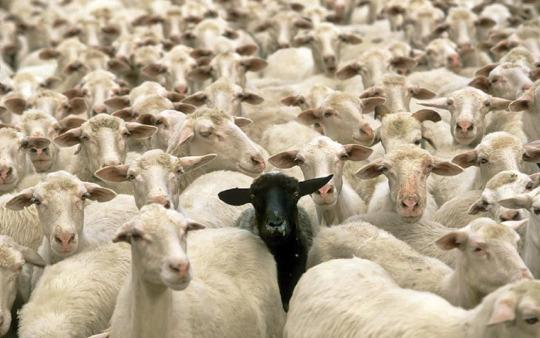
\includegraphics[height=3cm,width=3cm]{./Figures/sheep/sheep.jpg}
\caption{} 
\end{subfigure}\hspace*{\fill}
\begin{subfigure}{0.32\textwidth}
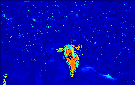
\includegraphics[height=3cm,width=3cm]{./Figures/sheep/1.png}
\caption{} 
\end{subfigure}
\begin{subfigure}{0.32\textwidth}
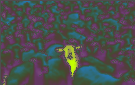
\includegraphics[height=3cm,width=3cm]{./Figures/sheep/2.png}
\caption{} 
\end{subfigure}

\medskip
\begin{subfigure}{0.32\textwidth}
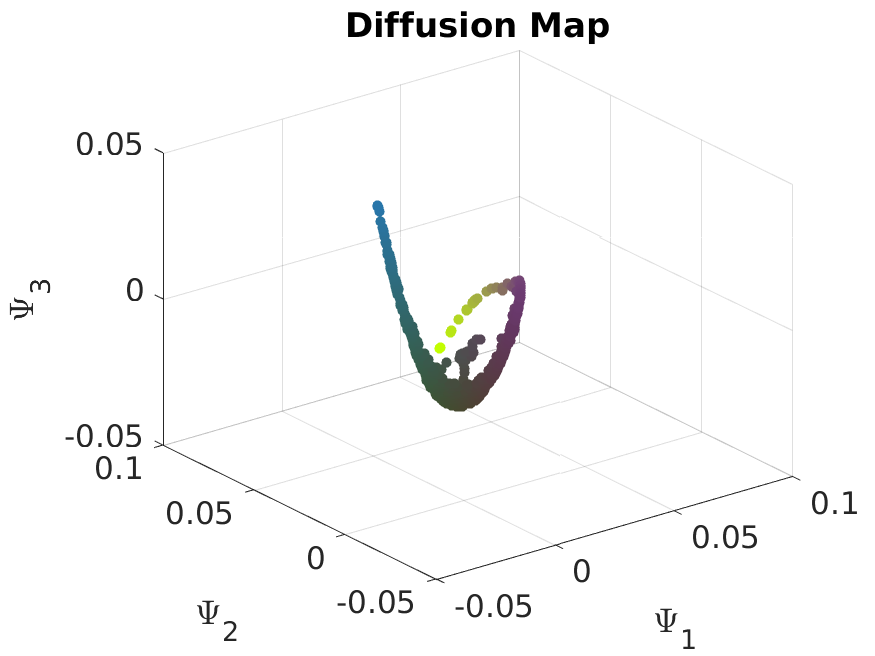
\includegraphics[height=3cm,width=3cm]{./Figures/sheep/3.png}
\caption{}
\end{subfigure}\hspace*{\fill}
\begin{subfigure}{0.32\textwidth}
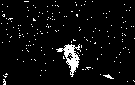
\includegraphics[height=3cm,width=3cm]{./Figures/sheep/5.png}
\caption{} 
\end{subfigure}
\begin{subfigure}{0.32\textwidth}
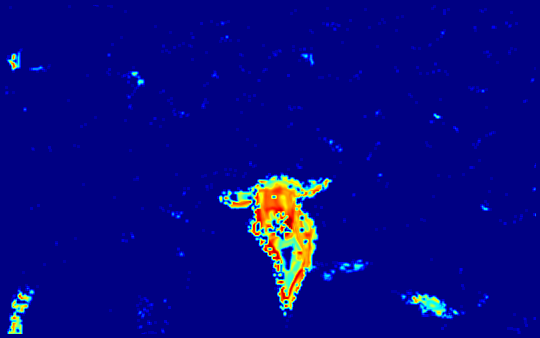
\includegraphics[height=3cm,width=3cm]{./Figures/sheep/6.png}
\caption{} 
\end{subfigure}

\caption{Anomaly Detection results for multiscale detector} \label{R:sheep}
\end{figure}


\begin{table}
\caption{Parameters used in Multiscle algorithms for figure \ref{fig:d} (Black Sheep)}
\begin{center}
 \begin{tabular}{c c c c c c c} 
  \hline\hline 
 $\mathbf{L}$ & Image & Patch & Window & Mask & Pixels (\%) & $\mathbf{d}$\\ [0.5ex]   
 \hline
 0 & $200\times200$ & $32\times32$ & $16\times16$ & $5\times5$ & 0.10 & 6 \\ 
 
 1 & $100\times100$ & $16\times16$ & $8\times8$ & $3\times3$ & 0.20 & 3 \\
 
 2 & $50\times50$ & $8\times8$ & $4\times4$ & $3\times3$ & 0.30 & 3 \\ [1ex] 
\hline
\end{tabular}
\end{center}
\label{T:sheep}
\end{table}
With positive results from above naive obvious black sheep image, we progress to other picture \ref{fig:c}. In this figure, the village girl is walking in the field. We have to detect her using our algorithms. Figure \ref{R:girl} visualizes our algorithms through different stage of algorithms. Corresponding parameters are summarized in Table \ref{T:sheep}.

\begin{figure}[t!] % "[t!]" placement specifier just for this example
\begin{subfigure}{0.32\textwidth}
\includegraphics[height=3cm,width=3cm]{./Figures/girl/girl.jpg}
\caption{} 
\end{subfigure}\hspace*{\fill}
\begin{subfigure}{0.32\textwidth}
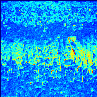
\includegraphics[height=3cm,width=3cm]{./Figures/girl/1.png}
\caption{} 
\end{subfigure}
\begin{subfigure}{0.32\textwidth}
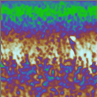
\includegraphics[height=3cm,width=3cm]{./Figures/girl/2.png}
\caption{} 
\end{subfigure}

\medskip
\begin{subfigure}{0.32\textwidth}
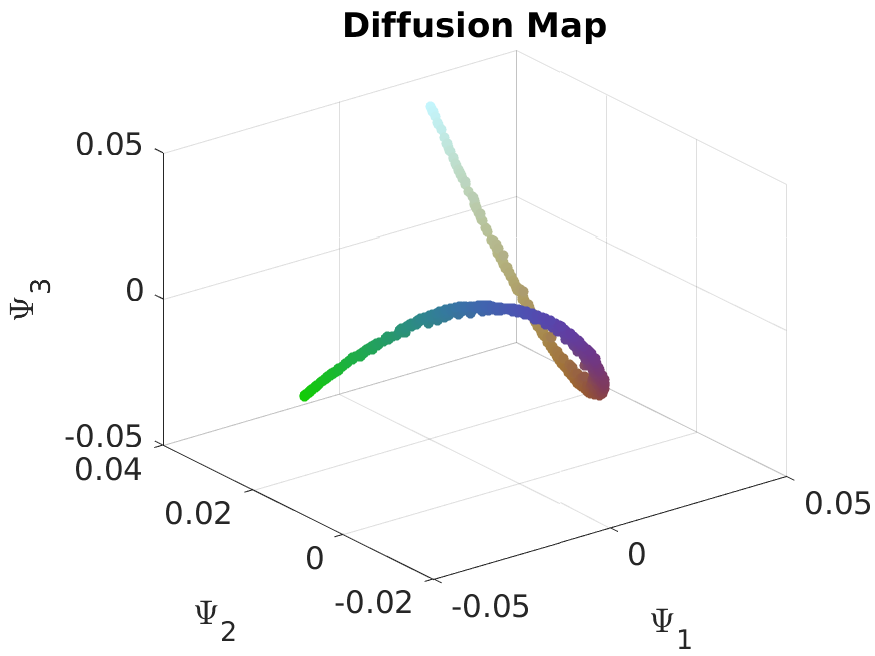
\includegraphics[height=3cm,width=3cm]{./Figures/girl/3.png}
\caption{}
\end{subfigure}\hspace*{\fill}
\begin{subfigure}{0.32\textwidth}
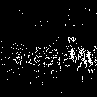
\includegraphics[height=3cm,width=3cm]{./Figures/girl/5.png}
\caption{} 
\end{subfigure}
\begin{subfigure}{0.32\textwidth}
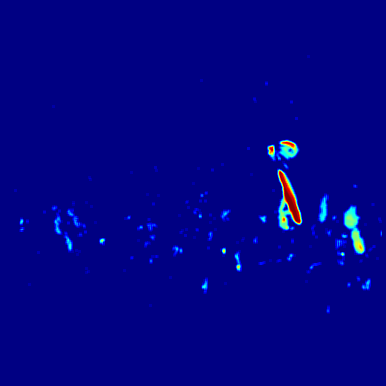
\includegraphics[height=3cm,width=3cm]{./Figures/girl/6.png}
\caption{} 
\end{subfigure}

\caption{Anomaly Detection results for multiscale detector} \label{R:girl}
\end{figure}

\begin{table}
\caption{Parameters used in Multiscle algorithms for figure \ref{fig:c} (Village Girl)}
\begin{center}
 \begin{tabular}{c c c c c c c} 
  \hline\hline 
 $\mathbf{L}$ & Image & Patch & Window & Mask & Pixels (\%) & $\mathbf{d}$\\ [0.5ex]   
 \hline
 0 & $200\times200$ & $8\times8$ & $40\times40$ & $6\times6$ & 0.10 & 6 \\ 
 
 1 & $100\times100$ & $4\times4$ & $20\times20$ & $3\times3$ & 0.30 & 3 \\
 
 2 & $50\times50$ & $2\times2$ & $10\times10$ & $2\times2$ & 0.50 & 3 \\ [1ex] 
\hline
\end{tabular}
\end{center}
\label{T:girl}
\end{table}

The image of village girl as anomaly was not contrast, so we take another image of girl standing in the field \ref{fig:e}. This image is more contrast  and larger in size as compared to village girl image. As the detections are found by thresholding the anomaly score image resulting in a binary image. Correct detection is considered as true positive and incorrect as false alarms. Unlike above two example, the proposed algorithms gives false alarms with the image where girls standing in the field is anomaly. Figure \ref{R:girlf} discuss the result for the image described. Table \ref{T:girlf} summarize the parameters.

\begin{figure}[t!] % "[t!]" placement specifier just for this example
\begin{subfigure}{0.32\textwidth}
\includegraphics[height=3cm,width=3cm]{./Figures/girlf/girlf.jpg}
\caption{} 
\end{subfigure}\hspace*{\fill}
\begin{subfigure}{0.32\textwidth}
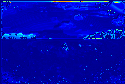
\includegraphics[height=3cm,width=3cm]{./Figures/girlf/1.png}
\caption{} 
\end{subfigure}
\begin{subfigure}{0.32\textwidth}
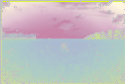
\includegraphics[height=3cm,width=3cm]{./Figures/girlf/2.png}
\caption{} 
\end{subfigure}

\medskip
\begin{subfigure}{0.32\textwidth}
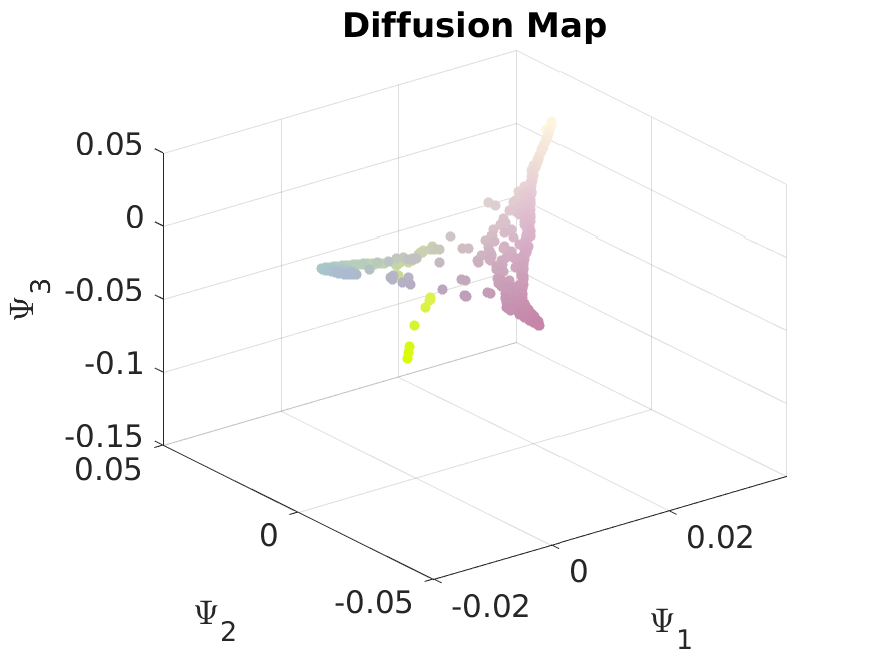
\includegraphics[height=3cm,width=3cm]{./Figures/girlf/3.png}
\caption{}
\end{subfigure}\hspace*{\fill}
\begin{subfigure}{0.32\textwidth}
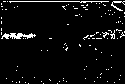
\includegraphics[height=3cm,width=3cm]{./Figures/girlf/5.png}
\caption{} 
\end{subfigure}
\begin{subfigure}{0.32\textwidth}
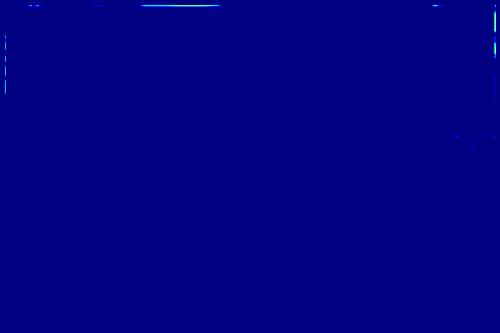
\includegraphics[height=3cm,width=3cm]{./Figures/girlf/6.png}
\caption{} 
\end{subfigure}

\caption{Anomaly Detection results for multiscale detector} \label{R:girlf}
\end{figure}

\begin{table}
\caption{Parameters used in Multiscle algorithms for figure \ref{fig:e} (girl in the field)}
\begin{center}
 \begin{tabular}{c c c c c c c} 
  \hline\hline 
 $\mathbf{L}$ & Image & Patch & Window & Mask & Pixels (\%) & $\mathbf{d}$\\ [0.5ex]   
 \hline
 
0 & $400\times400$ & $64\times64$ & $32\times32$ & $8\times8$ & 0.10 & 12 \\

 1 & $200\times200$ & $32\times32$ & $16\times16$ & $4\times4$ & 0.20 & 6 \\ 
 
 2 & $100\times100$ & $16\times16$ & $8\times8$ & $2\times2$ & 0.40 & 3 \\
 
 3 & $50\times50$ & $8\times8$ & $4\times4$ & $2\times2$ & 0.50 & 3 \\ [1ex] 
\hline
\end{tabular}
\end{center}
\label{T:girlf}
\end{table}

To replicate the results of the base paper\citep{Gal2013} for detection of sea-mines in side-scan sonar, we choose parameters as described in the Table \ref{T:sea}. Figure \ref{R:field} describe true positive results of proposed algorithm.

 
\begin{figure}[t!] % "[t!]" placement specifier just for this example
\begin{subfigure}{0.32\textwidth}
\includegraphics[height=3cm,width=3cm]{./Figures/field/field.jpg}
\caption{} 
\end{subfigure}\hspace*{\fill}
\begin{subfigure}{0.32\textwidth}
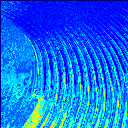
\includegraphics[height=3cm,width=3cm]{./Figures/field/1.png}
\caption{} 
\end{subfigure}
\begin{subfigure}{0.32\textwidth}
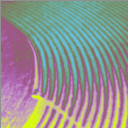
\includegraphics[height=3cm,width=3cm]{./Figures/field/2.png}
\caption{} 
\end{subfigure}

\medskip
\begin{subfigure}{0.32\textwidth}
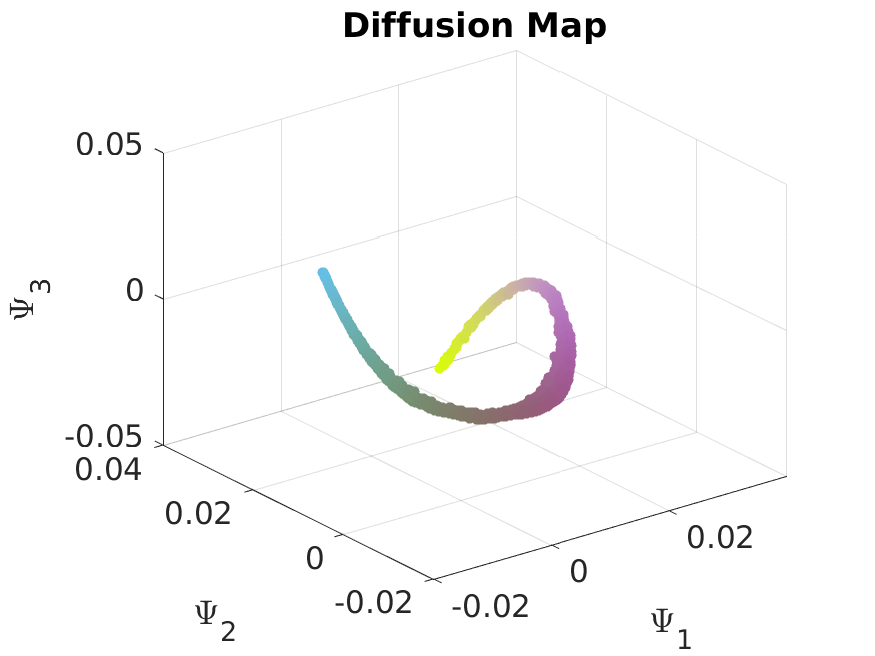
\includegraphics[height=3cm,width=3cm]{./Figures/field/3.png}
\caption{}
\end{subfigure}\hspace*{\fill}
\begin{subfigure}{0.32\textwidth}
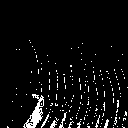
\includegraphics[height=3cm,width=3cm]{./Figures/field/5.png}
\caption{} 
\end{subfigure}
\begin{subfigure}{0.32\textwidth}
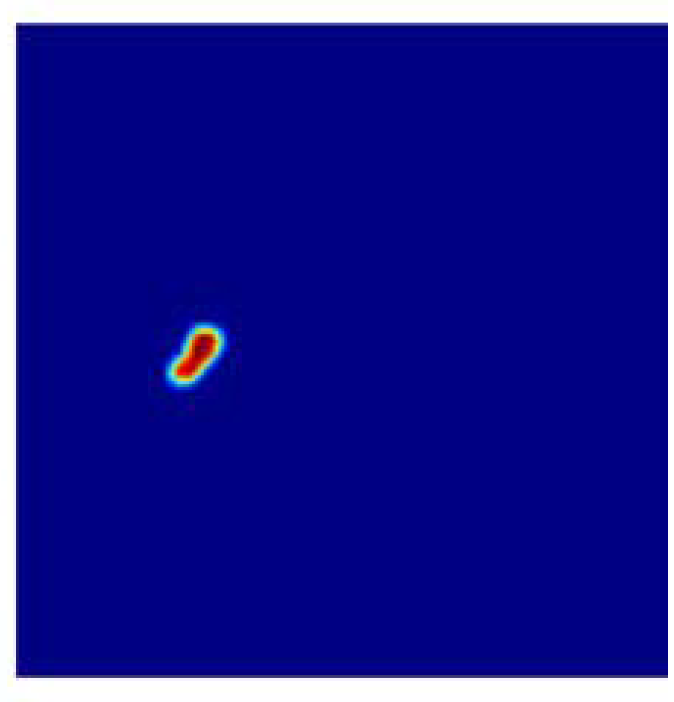
\includegraphics[height=3cm,width=3cm]{./Figures/field/6.png}
\caption{} 
\end{subfigure}

\caption{Anomaly Detection results for multiscale detector} \label{R:field}
\end{figure}

\begin{table}
\caption{Parameters used in Multiscle algorithms for figure \ref{fig:a} (sea-mines)}
\begin{center}
 \begin{tabular}{c c c c c c c} 
  \hline\hline 
 $\mathbf{L}$ & Image & Patch & Window & Mask & Pixels (\%) & $\mathbf{d}$\\ [0.5ex]   
 \hline
 0 & $200\times200$ & $8\times8$ & $41\times41$ & $9\times9$ & 0.10 & 6 \\ 
 
 1 & $100\times100$ & $4\times4$ & $21\times21$ & $5\times5$ & 0.33 & 3 \\
 
 2 & $50\times50$ & $2\times2$ & $13\times13$ & $5\times5$ & 0.50 & 3 \\ [1ex] 
\hline
\end{tabular}
\end{center}
\label{T:sea}
\end{table}

Our algorithm fails to give any results using figure \ref{fig:f}. This figure is of size $800\times800$ with very contrast background with multiple ducks which is hard to see. We have used the parameter as described in Table \ref{T: PD}.

\begin{table}
\caption{Parameters used in Multiscle algorithms for figure \ref{fig:f}}
\begin{center}
 \begin{tabular}{c c c c c c c} 
  \hline\hline 
 $\mathbf{L}$ & Image & Patch & Window & Mask & Pixels (\%) & $\mathbf{d}$\\ [0.5ex]   
 \hline
 0 & $800\times800$ & $128\times128$ & $64\times64$ & $18\times18$ & 0.10 & 24 \\ 

 1 & $400\times400$ & $64\times64$ & $32\times32$ & $9\times9$ & 0.20 & 12 \\

 2 & $200\times200$ & $32\times32$ & $16\times16$ & $5\times5$ & 0.30 & 6 \\ 
 
 3 & $100\times100$ & $16\times16$ & $8\times8$ & $3\times3$ & 0.40 & 3 \\
 
 4 & $50\times50$ & $8\times8$ & $4\times4$ & $3\times3$ & 0.50 & 3 \\ [1ex] 
\hline
\end{tabular}
\end{center}
\label{T: PD}
\end{table}

\section{Conclusions}
The proposed algorithms described in this chapter performs well the images which is not too contrast, but gives false positive on image which is of high resolutions. A future extension of this work would be combine  anomaly
scores from the different multiscale levels into a single anomaly score. This will enable detecting anomalies of different size in an image, which this algorithms fails to address.
